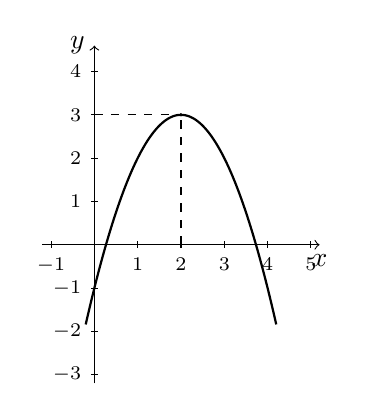
\begin{tikzpicture}[scale=0.55]
    \draw[->] (-1.2,0) -- (5.2,0) node[below] {$x$};
    \draw[->] (0,-3.2) -- (0,4.6) node[left] {$y$};
    \foreach \x in {-1,1,2,3,4,5}
        \draw (\x,0.08) -- (\x,-0.08) node[below] {\scriptsize $\x$};
    \foreach \y in {-3,-2,-1,1,2,3,4}
        \draw (0.08,\y) -- (-0.08,\y) node[left] {\scriptsize $\y$};
    \draw[smooth, samples=200, domain=-0.2:4.2, thick] plot (\x, {-(\x-2)^2+3});
    \fill (2,3) circle (1.2pt);
    \draw[dashed] (2,0) -- (2,3);
    \draw[dashed] (0,3) -- (2,3);
\end{tikzpicture}
